% Created by tikzDevice version 0.10.1 on 2016-07-18 19:10:49
% !TEX encoding = UTF-8 Unicode
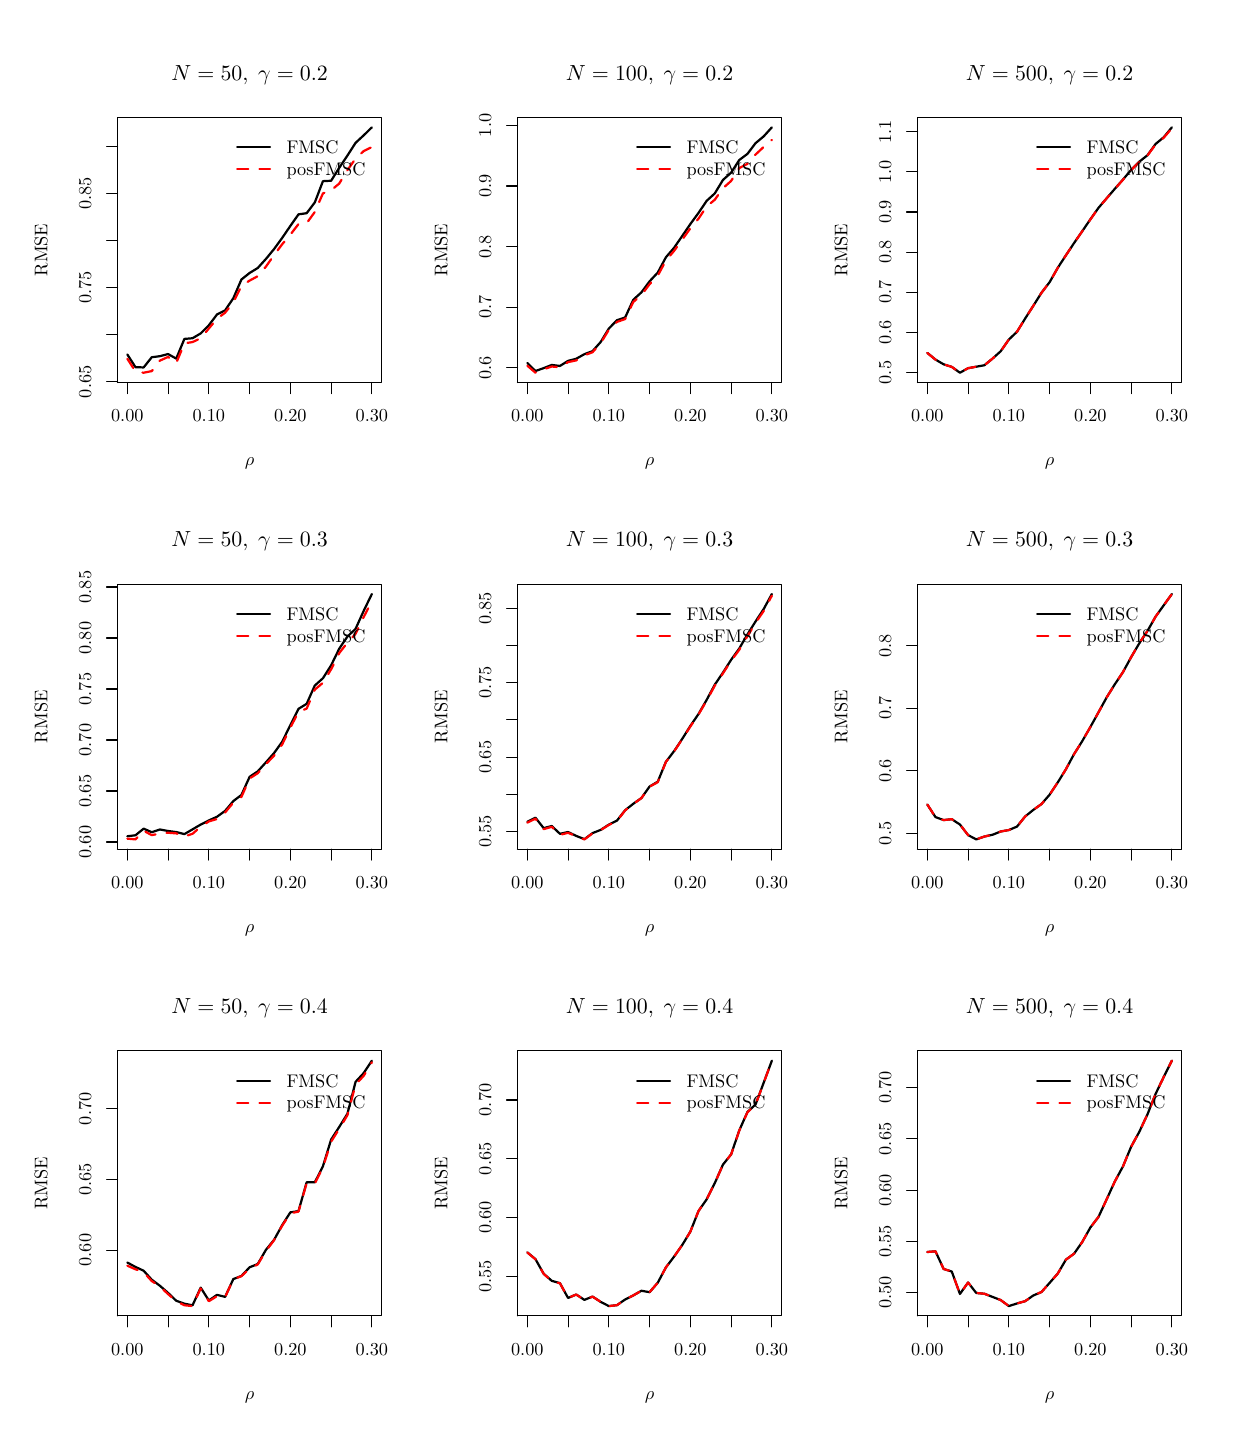
\begin{tikzpicture}[x=1pt,y=1pt]
\definecolor{fillColor}{RGB}{255,255,255}
\path[use as bounding box,fill=fillColor,fill opacity=0.00] (0,0) rectangle (433.62,505.89);
\begin{scope}
\path[clip] ( 32.47,377.65) rectangle (127.91,473.42);
\definecolor{drawColor}{RGB}{0,0,0}

\path[draw=drawColor,line width= 0.8pt,line join=round,line cap=round] ( 36.01,387.81) --
	( 38.95,383.21) --
	( 41.90,383.11) --
	( 44.84,386.80) --
	( 47.79,387.18) --
	( 50.73,387.95) --
	( 53.68,386.30) --
	( 56.63,393.42) --
	( 59.57,393.66) --
	( 62.52,395.41) --
	( 65.46,398.34) --
	( 68.41,402.25) --
	( 71.35,403.76) --
	( 74.30,408.09) --
	( 77.24,414.89) --
	( 80.19,417.24) --
	( 83.14,419.05) --
	( 86.08,422.30) --
	( 89.03,425.89) --
	( 91.97,429.92) --
	( 94.92,434.25) --
	( 97.86,438.43) --
	(100.81,438.85) --
	(103.75,442.73) --
	(106.70,450.43) --
	(109.65,450.57) --
	(112.59,455.27) --
	(115.54,459.67) --
	(118.48,464.26) --
	(121.43,466.99) --
	(124.37,469.87);
\end{scope}
\begin{scope}
\path[clip] (  0.00,  0.00) rectangle (433.62,505.89);
\definecolor{drawColor}{RGB}{0,0,0}

\path[draw=drawColor,line width= 0.4pt,line join=round,line cap=round] ( 36.01,377.65) -- (124.37,377.65);

\path[draw=drawColor,line width= 0.4pt,line join=round,line cap=round] ( 36.01,377.65) -- ( 36.01,373.69);

\path[draw=drawColor,line width= 0.4pt,line join=round,line cap=round] ( 50.73,377.65) -- ( 50.73,373.69);

\path[draw=drawColor,line width= 0.4pt,line join=round,line cap=round] ( 65.46,377.65) -- ( 65.46,373.69);

\path[draw=drawColor,line width= 0.4pt,line join=round,line cap=round] ( 80.19,377.65) -- ( 80.19,373.69);

\path[draw=drawColor,line width= 0.4pt,line join=round,line cap=round] ( 94.92,377.65) -- ( 94.92,373.69);

\path[draw=drawColor,line width= 0.4pt,line join=round,line cap=round] (109.65,377.65) -- (109.65,373.69);

\path[draw=drawColor,line width= 0.4pt,line join=round,line cap=round] (124.37,377.65) -- (124.37,373.69);

\node[text=drawColor,anchor=base,inner sep=0pt, outer sep=0pt, scale=  0.66] at ( 36.01,363.40) {0.00};

\node[text=drawColor,anchor=base,inner sep=0pt, outer sep=0pt, scale=  0.66] at ( 65.46,363.40) {0.10};

\node[text=drawColor,anchor=base,inner sep=0pt, outer sep=0pt, scale=  0.66] at ( 94.92,363.40) {0.20};

\node[text=drawColor,anchor=base,inner sep=0pt, outer sep=0pt, scale=  0.66] at (124.37,363.40) {0.30};

\path[draw=drawColor,line width= 0.4pt,line join=round,line cap=round] ( 32.47,377.93) -- ( 32.47,463.02);

\path[draw=drawColor,line width= 0.4pt,line join=round,line cap=round] ( 32.47,377.93) -- ( 28.51,377.93);

\path[draw=drawColor,line width= 0.4pt,line join=round,line cap=round] ( 32.47,394.94) -- ( 28.51,394.94);

\path[draw=drawColor,line width= 0.4pt,line join=round,line cap=round] ( 32.47,411.96) -- ( 28.51,411.96);

\path[draw=drawColor,line width= 0.4pt,line join=round,line cap=round] ( 32.47,428.98) -- ( 28.51,428.98);

\path[draw=drawColor,line width= 0.4pt,line join=round,line cap=round] ( 32.47,446.00) -- ( 28.51,446.00);

\path[draw=drawColor,line width= 0.4pt,line join=round,line cap=round] ( 32.47,463.02) -- ( 28.51,463.02);

\node[text=drawColor,rotate= 90.00,anchor=base,inner sep=0pt, outer sep=0pt, scale=  0.66] at ( 22.97,377.93) {0.65};

\node[text=drawColor,rotate= 90.00,anchor=base,inner sep=0pt, outer sep=0pt, scale=  0.66] at ( 22.97,411.96) {0.75};

\node[text=drawColor,rotate= 90.00,anchor=base,inner sep=0pt, outer sep=0pt, scale=  0.66] at ( 22.97,446.00) {0.85};

\path[draw=drawColor,line width= 0.4pt,line join=round,line cap=round] ( 32.47,377.65) --
	(127.91,377.65) --
	(127.91,473.42) --
	( 32.47,473.42) --
	( 32.47,377.65);
\end{scope}
\begin{scope}
\path[clip] (  0.00,337.26) rectangle (144.54,505.89);
\definecolor{drawColor}{RGB}{0,0,0}

\node[text=drawColor,anchor=base,inner sep=0pt, outer sep=0pt, scale=  0.79] at ( 80.19,486.92) {\bfseries $N=50, \;\gamma=0.2$};

\node[text=drawColor,anchor=base,inner sep=0pt, outer sep=0pt, scale=  0.66] at ( 80.19,347.56) {$\rho$};

\node[text=drawColor,rotate= 90.00,anchor=base,inner sep=0pt, outer sep=0pt, scale=  0.66] at (  7.13,425.53) {RMSE};
\end{scope}
\begin{scope}
\path[clip] ( 32.47,377.65) rectangle (127.91,473.42);
\definecolor{drawColor}{RGB}{255,0,0}

\path[draw=drawColor,line width= 0.8pt,dash pattern=on 4pt off 4pt ,line join=round,line cap=round] ( 36.01,386.26) --
	( 38.95,381.66) --
	( 41.90,381.20) --
	( 44.84,381.78) --
	( 47.79,385.58) --
	( 50.73,386.91) --
	( 53.68,384.71) --
	( 56.63,391.81) --
	( 59.57,392.28) --
	( 62.52,393.65) --
	( 65.46,397.18) --
	( 68.41,400.71) --
	( 71.35,402.90) --
	( 74.30,406.57) --
	( 77.24,412.58) --
	( 80.19,414.49) --
	( 83.14,416.08) --
	( 86.08,419.54) --
	( 89.03,423.70) --
	( 91.97,427.63) --
	( 94.92,431.10) --
	( 97.86,434.91) --
	(100.81,435.22) --
	(103.75,439.29) --
	(106.70,446.01) --
	(109.65,447.10) --
	(112.59,449.57) --
	(115.54,454.42) --
	(118.48,458.55) --
	(121.43,461.31) --
	(124.37,462.74);
\definecolor{drawColor}{RGB}{0,0,0}

\path[draw=drawColor,line width= 0.8pt,line join=round,line cap=round] ( 75.72,462.63) -- ( 87.60,462.63);
\definecolor{drawColor}{RGB}{255,0,0}

\path[draw=drawColor,line width= 0.8pt,dash pattern=on 4pt off 4pt ,line join=round,line cap=round] ( 75.72,454.71) -- ( 87.60,454.71);
\definecolor{drawColor}{RGB}{0,0,0}

\node[text=drawColor,anchor=base west,inner sep=0pt, outer sep=0pt, scale=  0.66] at ( 93.54,460.35) {FMSC};

\node[text=drawColor,anchor=base west,inner sep=0pt, outer sep=0pt, scale=  0.66] at ( 93.54,452.43) {posFMSC};
\end{scope}
\begin{scope}
\path[clip] (177.01,377.65) rectangle (272.45,473.42);
\definecolor{drawColor}{RGB}{0,0,0}

\path[draw=drawColor,line width= 0.8pt,line join=round,line cap=round] (180.55,384.71) --
	(183.49,381.82) --
	(186.44,382.86) --
	(189.38,384.01) --
	(192.33,383.65) --
	(195.27,385.48) --
	(198.22,386.25) --
	(201.17,387.91) --
	(204.11,389.00) --
	(207.06,392.31) --
	(210.00,397.16) --
	(212.95,400.19) --
	(215.89,401.16) --
	(218.84,407.57) --
	(221.78,410.25) --
	(224.73,414.23) --
	(227.68,417.40) --
	(230.62,422.91) --
	(233.57,426.34) --
	(236.51,430.60) --
	(239.46,434.93) --
	(242.40,438.94) --
	(245.35,443.31) --
	(248.29,446.00) --
	(251.24,450.86) --
	(254.19,453.50) --
	(257.13,458.06) --
	(260.08,460.27) --
	(263.02,464.16) --
	(265.97,466.62) --
	(268.91,469.87);
\end{scope}
\begin{scope}
\path[clip] (  0.00,  0.00) rectangle (433.62,505.89);
\definecolor{drawColor}{RGB}{0,0,0}

\path[draw=drawColor,line width= 0.4pt,line join=round,line cap=round] (180.55,377.65) -- (268.91,377.65);

\path[draw=drawColor,line width= 0.4pt,line join=round,line cap=round] (180.55,377.65) -- (180.55,373.69);

\path[draw=drawColor,line width= 0.4pt,line join=round,line cap=round] (195.27,377.65) -- (195.27,373.69);

\path[draw=drawColor,line width= 0.4pt,line join=round,line cap=round] (210.00,377.65) -- (210.00,373.69);

\path[draw=drawColor,line width= 0.4pt,line join=round,line cap=round] (224.73,377.65) -- (224.73,373.69);

\path[draw=drawColor,line width= 0.4pt,line join=round,line cap=round] (239.46,377.65) -- (239.46,373.69);

\path[draw=drawColor,line width= 0.4pt,line join=round,line cap=round] (254.19,377.65) -- (254.19,373.69);

\path[draw=drawColor,line width= 0.4pt,line join=round,line cap=round] (268.91,377.65) -- (268.91,373.69);

\node[text=drawColor,anchor=base,inner sep=0pt, outer sep=0pt, scale=  0.66] at (180.55,363.40) {0.00};

\node[text=drawColor,anchor=base,inner sep=0pt, outer sep=0pt, scale=  0.66] at (210.00,363.40) {0.10};

\node[text=drawColor,anchor=base,inner sep=0pt, outer sep=0pt, scale=  0.66] at (239.46,363.40) {0.20};

\node[text=drawColor,anchor=base,inner sep=0pt, outer sep=0pt, scale=  0.66] at (268.91,363.40) {0.30};

\path[draw=drawColor,line width= 0.4pt,line join=round,line cap=round] (177.01,382.96) -- (177.01,470.56);

\path[draw=drawColor,line width= 0.4pt,line join=round,line cap=round] (177.01,382.96) -- (173.05,382.96);

\path[draw=drawColor,line width= 0.4pt,line join=round,line cap=round] (177.01,404.86) -- (173.05,404.86);

\path[draw=drawColor,line width= 0.4pt,line join=round,line cap=round] (177.01,426.76) -- (173.05,426.76);

\path[draw=drawColor,line width= 0.4pt,line join=round,line cap=round] (177.01,448.66) -- (173.05,448.66);

\path[draw=drawColor,line width= 0.4pt,line join=round,line cap=round] (177.01,470.56) -- (173.05,470.56);

\node[text=drawColor,rotate= 90.00,anchor=base,inner sep=0pt, outer sep=0pt, scale=  0.66] at (167.51,382.96) {0.6};

\node[text=drawColor,rotate= 90.00,anchor=base,inner sep=0pt, outer sep=0pt, scale=  0.66] at (167.51,404.86) {0.7};

\node[text=drawColor,rotate= 90.00,anchor=base,inner sep=0pt, outer sep=0pt, scale=  0.66] at (167.51,426.76) {0.8};

\node[text=drawColor,rotate= 90.00,anchor=base,inner sep=0pt, outer sep=0pt, scale=  0.66] at (167.51,448.66) {0.9};

\node[text=drawColor,rotate= 90.00,anchor=base,inner sep=0pt, outer sep=0pt, scale=  0.66] at (167.51,470.56) {1.0};

\path[draw=drawColor,line width= 0.4pt,line join=round,line cap=round] (177.01,377.65) --
	(272.45,377.65) --
	(272.45,473.42) --
	(177.01,473.42) --
	(177.01,377.65);
\end{scope}
\begin{scope}
\path[clip] (144.54,337.26) rectangle (289.08,505.89);
\definecolor{drawColor}{RGB}{0,0,0}

\node[text=drawColor,anchor=base,inner sep=0pt, outer sep=0pt, scale=  0.79] at (224.73,486.92) {\bfseries $N=100, \;\gamma=0.2$};

\node[text=drawColor,anchor=base,inner sep=0pt, outer sep=0pt, scale=  0.66] at (224.73,347.56) {$\rho$};

\node[text=drawColor,rotate= 90.00,anchor=base,inner sep=0pt, outer sep=0pt, scale=  0.66] at (151.67,425.53) {RMSE};
\end{scope}
\begin{scope}
\path[clip] (177.01,377.65) rectangle (272.45,473.42);
\definecolor{drawColor}{RGB}{255,0,0}

\path[draw=drawColor,line width= 0.8pt,dash pattern=on 4pt off 4pt ,line join=round,line cap=round] (180.55,383.74) --
	(183.49,381.20) --
	(186.44,382.45) --
	(189.38,383.45) --
	(192.33,383.17) --
	(195.27,385.04) --
	(198.22,385.65) --
	(201.17,387.49) --
	(204.11,388.61) --
	(207.06,391.91) --
	(210.00,396.71) --
	(212.95,399.57) --
	(215.89,400.59) --
	(218.84,406.77) --
	(221.78,409.26) --
	(224.73,413.20) --
	(227.68,416.30) --
	(230.62,421.73) --
	(233.57,425.22) --
	(236.51,429.28) --
	(239.46,433.39) --
	(242.40,436.86) --
	(245.35,441.27) --
	(248.29,443.71) --
	(251.24,447.87) --
	(254.19,450.50) --
	(257.13,455.16) --
	(260.08,456.69) --
	(263.02,460.04) --
	(265.97,462.81) --
	(268.91,465.32);
\definecolor{drawColor}{RGB}{0,0,0}

\path[draw=drawColor,line width= 0.8pt,line join=round,line cap=round] (220.26,462.63) -- (232.14,462.63);
\definecolor{drawColor}{RGB}{255,0,0}

\path[draw=drawColor,line width= 0.8pt,dash pattern=on 4pt off 4pt ,line join=round,line cap=round] (220.26,454.71) -- (232.14,454.71);
\definecolor{drawColor}{RGB}{0,0,0}

\node[text=drawColor,anchor=base west,inner sep=0pt, outer sep=0pt, scale=  0.66] at (238.08,460.35) {FMSC};

\node[text=drawColor,anchor=base west,inner sep=0pt, outer sep=0pt, scale=  0.66] at (238.08,452.43) {posFMSC};
\end{scope}
\begin{scope}
\path[clip] (321.55,377.65) rectangle (416.99,473.42);
\definecolor{drawColor}{RGB}{0,0,0}

\path[draw=drawColor,line width= 0.8pt,line join=round,line cap=round] (325.09,388.37) --
	(328.03,385.95) --
	(330.98,384.24) --
	(333.92,383.32) --
	(336.87,381.20) --
	(339.81,382.84) --
	(342.76,383.38) --
	(345.71,383.90) --
	(348.65,386.31) --
	(351.60,388.96) --
	(354.54,393.19) --
	(357.49,396.00) --
	(360.43,400.78) --
	(363.38,405.38) --
	(366.32,410.07) --
	(369.27,413.92) --
	(372.22,419.12) --
	(375.16,423.63) --
	(378.11,428.07) --
	(381.05,432.31) --
	(384.00,436.64) --
	(386.94,440.78) --
	(389.89,444.24) --
	(392.83,447.64) --
	(395.78,450.99) --
	(398.73,454.50) --
	(401.67,457.46) --
	(404.62,459.77) --
	(407.56,463.85) --
	(410.51,466.29) --
	(413.45,469.87);
\end{scope}
\begin{scope}
\path[clip] (  0.00,  0.00) rectangle (433.62,505.89);
\definecolor{drawColor}{RGB}{0,0,0}

\path[draw=drawColor,line width= 0.4pt,line join=round,line cap=round] (325.09,377.65) -- (413.45,377.65);

\path[draw=drawColor,line width= 0.4pt,line join=round,line cap=round] (325.09,377.65) -- (325.09,373.69);

\path[draw=drawColor,line width= 0.4pt,line join=round,line cap=round] (339.81,377.65) -- (339.81,373.69);

\path[draw=drawColor,line width= 0.4pt,line join=round,line cap=round] (354.54,377.65) -- (354.54,373.69);

\path[draw=drawColor,line width= 0.4pt,line join=round,line cap=round] (369.27,377.65) -- (369.27,373.69);

\path[draw=drawColor,line width= 0.4pt,line join=round,line cap=round] (384.00,377.65) -- (384.00,373.69);

\path[draw=drawColor,line width= 0.4pt,line join=round,line cap=round] (398.73,377.65) -- (398.73,373.69);

\path[draw=drawColor,line width= 0.4pt,line join=round,line cap=round] (413.45,377.65) -- (413.45,373.69);

\node[text=drawColor,anchor=base,inner sep=0pt, outer sep=0pt, scale=  0.66] at (325.09,363.40) {0.00};

\node[text=drawColor,anchor=base,inner sep=0pt, outer sep=0pt, scale=  0.66] at (354.54,363.40) {0.10};

\node[text=drawColor,anchor=base,inner sep=0pt, outer sep=0pt, scale=  0.66] at (384.00,363.40) {0.20};

\node[text=drawColor,anchor=base,inner sep=0pt, outer sep=0pt, scale=  0.66] at (413.45,363.40) {0.30};

\path[draw=drawColor,line width= 0.4pt,line join=round,line cap=round] (321.55,381.29) -- (321.55,468.27);

\path[draw=drawColor,line width= 0.4pt,line join=round,line cap=round] (321.55,381.29) -- (317.59,381.29);

\path[draw=drawColor,line width= 0.4pt,line join=round,line cap=round] (321.55,395.78) -- (317.59,395.78);

\path[draw=drawColor,line width= 0.4pt,line join=round,line cap=round] (321.55,410.28) -- (317.59,410.28);

\path[draw=drawColor,line width= 0.4pt,line join=round,line cap=round] (321.55,424.78) -- (317.59,424.78);

\path[draw=drawColor,line width= 0.4pt,line join=round,line cap=round] (321.55,439.27) -- (317.59,439.27);

\path[draw=drawColor,line width= 0.4pt,line join=round,line cap=round] (321.55,453.77) -- (317.59,453.77);

\path[draw=drawColor,line width= 0.4pt,line join=round,line cap=round] (321.55,468.27) -- (317.59,468.27);

\node[text=drawColor,rotate= 90.00,anchor=base,inner sep=0pt, outer sep=0pt, scale=  0.66] at (312.05,381.29) {0.5};

\node[text=drawColor,rotate= 90.00,anchor=base,inner sep=0pt, outer sep=0pt, scale=  0.66] at (312.05,395.78) {0.6};

\node[text=drawColor,rotate= 90.00,anchor=base,inner sep=0pt, outer sep=0pt, scale=  0.66] at (312.05,410.28) {0.7};

\node[text=drawColor,rotate= 90.00,anchor=base,inner sep=0pt, outer sep=0pt, scale=  0.66] at (312.05,424.78) {0.8};

\node[text=drawColor,rotate= 90.00,anchor=base,inner sep=0pt, outer sep=0pt, scale=  0.66] at (312.05,439.27) {0.9};

\node[text=drawColor,rotate= 90.00,anchor=base,inner sep=0pt, outer sep=0pt, scale=  0.66] at (312.05,453.77) {1.0};

\node[text=drawColor,rotate= 90.00,anchor=base,inner sep=0pt, outer sep=0pt, scale=  0.66] at (312.05,468.27) {1.1};

\path[draw=drawColor,line width= 0.4pt,line join=round,line cap=round] (321.55,377.65) --
	(416.99,377.65) --
	(416.99,473.42) --
	(321.55,473.42) --
	(321.55,377.65);
\end{scope}
\begin{scope}
\path[clip] (289.08,337.26) rectangle (433.62,505.89);
\definecolor{drawColor}{RGB}{0,0,0}

\node[text=drawColor,anchor=base,inner sep=0pt, outer sep=0pt, scale=  0.79] at (369.27,486.92) {\bfseries $N=500, \;\gamma=0.2$};

\node[text=drawColor,anchor=base,inner sep=0pt, outer sep=0pt, scale=  0.66] at (369.27,347.56) {$\rho$};

\node[text=drawColor,rotate= 90.00,anchor=base,inner sep=0pt, outer sep=0pt, scale=  0.66] at (296.21,425.53) {RMSE};
\end{scope}
\begin{scope}
\path[clip] (321.55,377.65) rectangle (416.99,473.42);
\definecolor{drawColor}{RGB}{255,0,0}

\path[draw=drawColor,line width= 0.8pt,dash pattern=on 4pt off 4pt ,line join=round,line cap=round] (325.09,388.35) --
	(328.03,385.94) --
	(330.98,384.23) --
	(333.92,383.31) --
	(336.87,381.20) --
	(339.81,382.84) --
	(342.76,383.38) --
	(345.71,383.89) --
	(348.65,386.31) --
	(351.60,388.96) --
	(354.54,393.19) --
	(357.49,396.00) --
	(360.43,400.78) --
	(363.38,405.38) --
	(366.32,410.06) --
	(369.27,413.92) --
	(372.22,419.09) --
	(375.16,423.62) --
	(378.11,428.07) --
	(381.05,432.31) --
	(384.00,436.56) --
	(386.94,440.77) --
	(389.89,444.20) --
	(392.83,447.58) --
	(395.78,450.94) --
	(398.73,454.39) --
	(401.67,457.37) --
	(404.62,459.68) --
	(407.56,463.65) --
	(410.51,466.12) --
	(413.45,469.52);
\definecolor{drawColor}{RGB}{0,0,0}

\path[draw=drawColor,line width= 0.8pt,line join=round,line cap=round] (364.80,462.63) -- (376.68,462.63);
\definecolor{drawColor}{RGB}{255,0,0}

\path[draw=drawColor,line width= 0.8pt,dash pattern=on 4pt off 4pt ,line join=round,line cap=round] (364.80,454.71) -- (376.68,454.71);
\definecolor{drawColor}{RGB}{0,0,0}

\node[text=drawColor,anchor=base west,inner sep=0pt, outer sep=0pt, scale=  0.66] at (382.62,460.35) {FMSC};

\node[text=drawColor,anchor=base west,inner sep=0pt, outer sep=0pt, scale=  0.66] at (382.62,452.43) {posFMSC};
\end{scope}
\begin{scope}
\path[clip] ( 32.47,209.02) rectangle (127.91,304.79);
\definecolor{drawColor}{RGB}{0,0,0}

\path[draw=drawColor,line width= 0.8pt,line join=round,line cap=round] ( 36.01,213.71) --
	( 38.95,214.06) --
	( 41.90,216.45) --
	( 44.84,215.17) --
	( 47.79,216.15) --
	( 50.73,215.61) --
	( 53.68,215.22) --
	( 56.63,214.48) --
	( 59.57,216.20) --
	( 62.52,217.93) --
	( 65.46,219.42) --
	( 68.41,220.75) --
	( 71.35,222.88) --
	( 74.30,226.41) --
	( 77.24,228.63) --
	( 80.19,235.17) --
	( 83.14,237.16) --
	( 86.08,240.40) --
	( 89.03,243.77) --
	( 91.97,247.85) --
	( 94.92,253.89) --
	( 97.86,259.75) --
	(100.81,261.56) --
	(103.75,268.16) --
	(106.70,270.81) --
	(109.65,275.47) --
	(112.59,281.51) --
	(115.54,285.86) --
	(118.48,288.64) --
	(121.43,295.18) --
	(124.37,301.24);
\end{scope}
\begin{scope}
\path[clip] (  0.00,  0.00) rectangle (433.62,505.89);
\definecolor{drawColor}{RGB}{0,0,0}

\path[draw=drawColor,line width= 0.4pt,line join=round,line cap=round] ( 36.01,209.02) -- (124.37,209.02);

\path[draw=drawColor,line width= 0.4pt,line join=round,line cap=round] ( 36.01,209.02) -- ( 36.01,205.06);

\path[draw=drawColor,line width= 0.4pt,line join=round,line cap=round] ( 50.73,209.02) -- ( 50.73,205.06);

\path[draw=drawColor,line width= 0.4pt,line join=round,line cap=round] ( 65.46,209.02) -- ( 65.46,205.06);

\path[draw=drawColor,line width= 0.4pt,line join=round,line cap=round] ( 80.19,209.02) -- ( 80.19,205.06);

\path[draw=drawColor,line width= 0.4pt,line join=round,line cap=round] ( 94.92,209.02) -- ( 94.92,205.06);

\path[draw=drawColor,line width= 0.4pt,line join=round,line cap=round] (109.65,209.02) -- (109.65,205.06);

\path[draw=drawColor,line width= 0.4pt,line join=round,line cap=round] (124.37,209.02) -- (124.37,205.06);

\node[text=drawColor,anchor=base,inner sep=0pt, outer sep=0pt, scale=  0.66] at ( 36.01,194.77) {0.00};

\node[text=drawColor,anchor=base,inner sep=0pt, outer sep=0pt, scale=  0.66] at ( 65.46,194.77) {0.10};

\node[text=drawColor,anchor=base,inner sep=0pt, outer sep=0pt, scale=  0.66] at ( 94.92,194.77) {0.20};

\node[text=drawColor,anchor=base,inner sep=0pt, outer sep=0pt, scale=  0.66] at (124.37,194.77) {0.30};

\path[draw=drawColor,line width= 0.4pt,line join=round,line cap=round] ( 32.47,211.64) -- ( 32.47,303.77);

\path[draw=drawColor,line width= 0.4pt,line join=round,line cap=round] ( 32.47,211.64) -- ( 28.51,211.64);

\path[draw=drawColor,line width= 0.4pt,line join=round,line cap=round] ( 32.47,230.06) -- ( 28.51,230.06);

\path[draw=drawColor,line width= 0.4pt,line join=round,line cap=round] ( 32.47,248.49) -- ( 28.51,248.49);

\path[draw=drawColor,line width= 0.4pt,line join=round,line cap=round] ( 32.47,266.92) -- ( 28.51,266.92);

\path[draw=drawColor,line width= 0.4pt,line join=round,line cap=round] ( 32.47,285.34) -- ( 28.51,285.34);

\path[draw=drawColor,line width= 0.4pt,line join=round,line cap=round] ( 32.47,303.77) -- ( 28.51,303.77);

\node[text=drawColor,rotate= 90.00,anchor=base,inner sep=0pt, outer sep=0pt, scale=  0.66] at ( 22.97,211.64) {0.60};

\node[text=drawColor,rotate= 90.00,anchor=base,inner sep=0pt, outer sep=0pt, scale=  0.66] at ( 22.97,230.06) {0.65};

\node[text=drawColor,rotate= 90.00,anchor=base,inner sep=0pt, outer sep=0pt, scale=  0.66] at ( 22.97,248.49) {0.70};

\node[text=drawColor,rotate= 90.00,anchor=base,inner sep=0pt, outer sep=0pt, scale=  0.66] at ( 22.97,266.92) {0.75};

\node[text=drawColor,rotate= 90.00,anchor=base,inner sep=0pt, outer sep=0pt, scale=  0.66] at ( 22.97,285.34) {0.80};

\node[text=drawColor,rotate= 90.00,anchor=base,inner sep=0pt, outer sep=0pt, scale=  0.66] at ( 22.97,303.77) {0.85};

\path[draw=drawColor,line width= 0.4pt,line join=round,line cap=round] ( 32.47,209.02) --
	(127.91,209.02) --
	(127.91,304.79) --
	( 32.47,304.79) --
	( 32.47,209.02);
\end{scope}
\begin{scope}
\path[clip] (  0.00,168.63) rectangle (144.54,337.26);
\definecolor{drawColor}{RGB}{0,0,0}

\node[text=drawColor,anchor=base,inner sep=0pt, outer sep=0pt, scale=  0.79] at ( 80.19,318.29) {\bfseries $N=50, \;\gamma=0.3$};

\node[text=drawColor,anchor=base,inner sep=0pt, outer sep=0pt, scale=  0.66] at ( 80.19,178.93) {$\rho$};

\node[text=drawColor,rotate= 90.00,anchor=base,inner sep=0pt, outer sep=0pt, scale=  0.66] at (  7.13,256.90) {RMSE};
\end{scope}
\begin{scope}
\path[clip] ( 32.47,209.02) rectangle (127.91,304.79);
\definecolor{drawColor}{RGB}{255,0,0}

\path[draw=drawColor,line width= 0.8pt,dash pattern=on 4pt off 4pt ,line join=round,line cap=round] ( 36.01,212.84) --
	( 38.95,212.57) --
	( 41.90,215.70) --
	( 44.84,214.10) --
	( 47.79,214.72) --
	( 50.73,214.97) --
	( 53.68,214.75) --
	( 56.63,213.63) --
	( 59.57,214.60) --
	( 62.52,217.15) --
	( 65.46,219.06) --
	( 68.41,219.95) --
	( 71.35,222.31) --
	( 74.30,225.86) --
	( 77.24,227.92) --
	( 80.19,234.59) --
	( 83.14,236.49) --
	( 86.08,239.75) --
	( 89.03,242.82) --
	( 91.97,246.89) --
	( 94.92,252.98) --
	( 97.86,258.65) --
	(100.81,259.83) --
	(103.75,266.69) --
	(106.70,269.16) --
	(109.65,274.04) --
	(112.59,279.91) --
	(115.54,283.66) --
	(118.48,286.84) --
	(121.43,292.93) --
	(124.37,298.65);
\definecolor{drawColor}{RGB}{0,0,0}

\path[draw=drawColor,line width= 0.8pt,line join=round,line cap=round] ( 75.72,294.00) -- ( 87.60,294.00);
\definecolor{drawColor}{RGB}{255,0,0}

\path[draw=drawColor,line width= 0.8pt,dash pattern=on 4pt off 4pt ,line join=round,line cap=round] ( 75.72,286.08) -- ( 87.60,286.08);
\definecolor{drawColor}{RGB}{0,0,0}

\node[text=drawColor,anchor=base west,inner sep=0pt, outer sep=0pt, scale=  0.66] at ( 93.54,291.72) {FMSC};

\node[text=drawColor,anchor=base west,inner sep=0pt, outer sep=0pt, scale=  0.66] at ( 93.54,283.80) {posFMSC};
\end{scope}
\begin{scope}
\path[clip] (177.01,209.02) rectangle (272.45,304.79);
\definecolor{drawColor}{RGB}{0,0,0}

\path[draw=drawColor,line width= 0.8pt,line join=round,line cap=round] (180.55,218.95) --
	(183.49,220.41) --
	(186.44,216.64) --
	(189.38,217.41) --
	(192.33,214.59) --
	(195.27,215.23) --
	(198.22,213.83) --
	(201.17,212.66) --
	(204.11,214.84) --
	(207.06,216.01) --
	(210.00,217.91) --
	(212.95,219.37) --
	(215.89,223.11) --
	(218.84,225.45) --
	(221.78,227.52) --
	(224.73,231.69) --
	(227.68,233.42) --
	(230.62,240.61) --
	(233.57,244.45) --
	(236.51,248.87) --
	(239.46,253.58) --
	(242.40,257.87) --
	(245.35,262.99) --
	(248.29,268.49) --
	(251.24,272.84) --
	(254.19,277.47) --
	(257.13,281.55) --
	(260.08,286.62) --
	(263.02,291.33) --
	(265.97,295.83) --
	(268.91,301.24);
\end{scope}
\begin{scope}
\path[clip] (  0.00,  0.00) rectangle (433.62,505.89);
\definecolor{drawColor}{RGB}{0,0,0}

\path[draw=drawColor,line width= 0.4pt,line join=round,line cap=round] (180.55,209.02) -- (268.91,209.02);

\path[draw=drawColor,line width= 0.4pt,line join=round,line cap=round] (180.55,209.02) -- (180.55,205.06);

\path[draw=drawColor,line width= 0.4pt,line join=round,line cap=round] (195.27,209.02) -- (195.27,205.06);

\path[draw=drawColor,line width= 0.4pt,line join=round,line cap=round] (210.00,209.02) -- (210.00,205.06);

\path[draw=drawColor,line width= 0.4pt,line join=round,line cap=round] (224.73,209.02) -- (224.73,205.06);

\path[draw=drawColor,line width= 0.4pt,line join=round,line cap=round] (239.46,209.02) -- (239.46,205.06);

\path[draw=drawColor,line width= 0.4pt,line join=round,line cap=round] (254.19,209.02) -- (254.19,205.06);

\path[draw=drawColor,line width= 0.4pt,line join=round,line cap=round] (268.91,209.02) -- (268.91,205.06);

\node[text=drawColor,anchor=base,inner sep=0pt, outer sep=0pt, scale=  0.66] at (180.55,194.77) {0.00};

\node[text=drawColor,anchor=base,inner sep=0pt, outer sep=0pt, scale=  0.66] at (210.00,194.77) {0.10};

\node[text=drawColor,anchor=base,inner sep=0pt, outer sep=0pt, scale=  0.66] at (239.46,194.77) {0.20};

\node[text=drawColor,anchor=base,inner sep=0pt, outer sep=0pt, scale=  0.66] at (268.91,194.77) {0.30};

\path[draw=drawColor,line width= 0.4pt,line join=round,line cap=round] (177.01,215.45) -- (177.01,296.06);

\path[draw=drawColor,line width= 0.4pt,line join=round,line cap=round] (177.01,215.45) -- (173.05,215.45);

\path[draw=drawColor,line width= 0.4pt,line join=round,line cap=round] (177.01,228.88) -- (173.05,228.88);

\path[draw=drawColor,line width= 0.4pt,line join=round,line cap=round] (177.01,242.32) -- (173.05,242.32);

\path[draw=drawColor,line width= 0.4pt,line join=round,line cap=round] (177.01,255.75) -- (173.05,255.75);

\path[draw=drawColor,line width= 0.4pt,line join=round,line cap=round] (177.01,269.19) -- (173.05,269.19);

\path[draw=drawColor,line width= 0.4pt,line join=round,line cap=round] (177.01,282.62) -- (173.05,282.62);

\path[draw=drawColor,line width= 0.4pt,line join=round,line cap=round] (177.01,296.06) -- (173.05,296.06);

\node[text=drawColor,rotate= 90.00,anchor=base,inner sep=0pt, outer sep=0pt, scale=  0.66] at (167.51,215.45) {0.55};

\node[text=drawColor,rotate= 90.00,anchor=base,inner sep=0pt, outer sep=0pt, scale=  0.66] at (167.51,242.32) {0.65};

\node[text=drawColor,rotate= 90.00,anchor=base,inner sep=0pt, outer sep=0pt, scale=  0.66] at (167.51,269.19) {0.75};

\node[text=drawColor,rotate= 90.00,anchor=base,inner sep=0pt, outer sep=0pt, scale=  0.66] at (167.51,296.06) {0.85};

\path[draw=drawColor,line width= 0.4pt,line join=round,line cap=round] (177.01,209.02) --
	(272.45,209.02) --
	(272.45,304.79) --
	(177.01,304.79) --
	(177.01,209.02);
\end{scope}
\begin{scope}
\path[clip] (144.54,168.63) rectangle (289.08,337.26);
\definecolor{drawColor}{RGB}{0,0,0}

\node[text=drawColor,anchor=base,inner sep=0pt, outer sep=0pt, scale=  0.79] at (224.73,318.29) {\bfseries $N=100, \;\gamma=0.3$};

\node[text=drawColor,anchor=base,inner sep=0pt, outer sep=0pt, scale=  0.66] at (224.73,178.93) {$\rho$};

\node[text=drawColor,rotate= 90.00,anchor=base,inner sep=0pt, outer sep=0pt, scale=  0.66] at (151.67,256.90) {RMSE};
\end{scope}
\begin{scope}
\path[clip] (177.01,209.02) rectangle (272.45,304.79);
\definecolor{drawColor}{RGB}{255,0,0}

\path[draw=drawColor,line width= 0.8pt,dash pattern=on 4pt off 4pt ,line join=round,line cap=round] (180.55,218.62) --
	(183.49,220.06) --
	(186.44,216.27) --
	(189.38,217.12) --
	(192.33,214.21) --
	(195.27,214.94) --
	(198.22,213.75) --
	(201.17,212.57) --
	(204.11,214.77) --
	(207.06,215.93) --
	(210.00,217.79) --
	(212.95,219.24) --
	(215.89,223.05) --
	(218.84,225.36) --
	(221.78,227.49) --
	(224.73,231.63) --
	(227.68,233.24) --
	(230.62,240.57) --
	(233.57,244.31) --
	(236.51,248.79) --
	(239.46,253.37) --
	(242.40,257.70) --
	(245.35,262.75) --
	(248.29,268.12) --
	(251.24,272.58) --
	(254.19,277.11) --
	(257.13,281.09) --
	(260.08,285.97) --
	(263.02,290.81) --
	(265.97,295.15) --
	(268.91,300.64);
\definecolor{drawColor}{RGB}{0,0,0}

\path[draw=drawColor,line width= 0.8pt,line join=round,line cap=round] (220.26,294.00) -- (232.14,294.00);
\definecolor{drawColor}{RGB}{255,0,0}

\path[draw=drawColor,line width= 0.8pt,dash pattern=on 4pt off 4pt ,line join=round,line cap=round] (220.26,286.08) -- (232.14,286.08);
\definecolor{drawColor}{RGB}{0,0,0}

\node[text=drawColor,anchor=base west,inner sep=0pt, outer sep=0pt, scale=  0.66] at (238.08,291.72) {FMSC};

\node[text=drawColor,anchor=base west,inner sep=0pt, outer sep=0pt, scale=  0.66] at (238.08,283.80) {posFMSC};
\end{scope}
\begin{scope}
\path[clip] (321.55,209.02) rectangle (416.99,304.79);
\definecolor{drawColor}{RGB}{0,0,0}

\path[draw=drawColor,line width= 0.8pt,line join=round,line cap=round] (325.09,225.15) --
	(328.03,220.63) --
	(330.98,219.55) --
	(333.92,219.87) --
	(336.87,217.95) --
	(339.81,214.13) --
	(342.76,212.57) --
	(345.71,213.61) --
	(348.65,214.25) --
	(351.60,215.43) --
	(354.54,215.95) --
	(357.49,217.20) --
	(360.43,220.85) --
	(363.38,223.23) --
	(366.32,225.33) --
	(369.27,228.72) --
	(372.22,233.16) --
	(375.16,237.92) --
	(378.11,243.40) --
	(381.05,248.06) --
	(384.00,253.18) --
	(386.94,258.50) --
	(389.89,263.88) --
	(392.83,268.62) --
	(395.78,273.02) --
	(398.73,278.42) --
	(401.67,283.41) --
	(404.62,287.86) --
	(407.56,293.06) --
	(410.51,297.16) --
	(413.45,301.24);
\end{scope}
\begin{scope}
\path[clip] (  0.00,  0.00) rectangle (433.62,505.89);
\definecolor{drawColor}{RGB}{0,0,0}

\path[draw=drawColor,line width= 0.4pt,line join=round,line cap=round] (325.09,209.02) -- (413.45,209.02);

\path[draw=drawColor,line width= 0.4pt,line join=round,line cap=round] (325.09,209.02) -- (325.09,205.06);

\path[draw=drawColor,line width= 0.4pt,line join=round,line cap=round] (339.81,209.02) -- (339.81,205.06);

\path[draw=drawColor,line width= 0.4pt,line join=round,line cap=round] (354.54,209.02) -- (354.54,205.06);

\path[draw=drawColor,line width= 0.4pt,line join=round,line cap=round] (369.27,209.02) -- (369.27,205.06);

\path[draw=drawColor,line width= 0.4pt,line join=round,line cap=round] (384.00,209.02) -- (384.00,205.06);

\path[draw=drawColor,line width= 0.4pt,line join=round,line cap=round] (398.73,209.02) -- (398.73,205.06);

\path[draw=drawColor,line width= 0.4pt,line join=round,line cap=round] (413.45,209.02) -- (413.45,205.06);

\node[text=drawColor,anchor=base,inner sep=0pt, outer sep=0pt, scale=  0.66] at (325.09,194.77) {0.00};

\node[text=drawColor,anchor=base,inner sep=0pt, outer sep=0pt, scale=  0.66] at (354.54,194.77) {0.10};

\node[text=drawColor,anchor=base,inner sep=0pt, outer sep=0pt, scale=  0.66] at (384.00,194.77) {0.20};

\node[text=drawColor,anchor=base,inner sep=0pt, outer sep=0pt, scale=  0.66] at (413.45,194.77) {0.30};

\path[draw=drawColor,line width= 0.4pt,line join=round,line cap=round] (321.55,214.73) -- (321.55,282.56);

\path[draw=drawColor,line width= 0.4pt,line join=round,line cap=round] (321.55,214.73) -- (317.59,214.73);

\path[draw=drawColor,line width= 0.4pt,line join=round,line cap=round] (321.55,237.34) -- (317.59,237.34);

\path[draw=drawColor,line width= 0.4pt,line join=round,line cap=round] (321.55,259.95) -- (317.59,259.95);

\path[draw=drawColor,line width= 0.4pt,line join=round,line cap=round] (321.55,282.56) -- (317.59,282.56);

\node[text=drawColor,rotate= 90.00,anchor=base,inner sep=0pt, outer sep=0pt, scale=  0.66] at (312.05,214.73) {0.5};

\node[text=drawColor,rotate= 90.00,anchor=base,inner sep=0pt, outer sep=0pt, scale=  0.66] at (312.05,237.34) {0.6};

\node[text=drawColor,rotate= 90.00,anchor=base,inner sep=0pt, outer sep=0pt, scale=  0.66] at (312.05,259.95) {0.7};

\node[text=drawColor,rotate= 90.00,anchor=base,inner sep=0pt, outer sep=0pt, scale=  0.66] at (312.05,282.56) {0.8};

\path[draw=drawColor,line width= 0.4pt,line join=round,line cap=round] (321.55,209.02) --
	(416.99,209.02) --
	(416.99,304.79) --
	(321.55,304.79) --
	(321.55,209.02);
\end{scope}
\begin{scope}
\path[clip] (289.08,168.63) rectangle (433.62,337.26);
\definecolor{drawColor}{RGB}{0,0,0}

\node[text=drawColor,anchor=base,inner sep=0pt, outer sep=0pt, scale=  0.79] at (369.27,318.29) {\bfseries $N=500, \;\gamma=0.3$};

\node[text=drawColor,anchor=base,inner sep=0pt, outer sep=0pt, scale=  0.66] at (369.27,178.93) {$\rho$};

\node[text=drawColor,rotate= 90.00,anchor=base,inner sep=0pt, outer sep=0pt, scale=  0.66] at (296.21,256.90) {RMSE};
\end{scope}
\begin{scope}
\path[clip] (321.55,209.02) rectangle (416.99,304.79);
\definecolor{drawColor}{RGB}{255,0,0}

\path[draw=drawColor,line width= 0.8pt,dash pattern=on 4pt off 4pt ,line join=round,line cap=round] (325.09,225.15) --
	(328.03,220.63) --
	(330.98,219.55) --
	(333.92,219.87) --
	(336.87,217.95) --
	(339.81,214.13) --
	(342.76,212.57) --
	(345.71,213.61) --
	(348.65,214.25) --
	(351.60,215.43) --
	(354.54,215.95) --
	(357.49,217.20) --
	(360.43,220.85) --
	(363.38,223.23) --
	(366.32,225.33) --
	(369.27,228.72) --
	(372.22,233.16) --
	(375.16,237.92) --
	(378.11,243.40) --
	(381.05,248.06) --
	(384.00,253.18) --
	(386.94,258.50) --
	(389.89,263.88) --
	(392.83,268.62) --
	(395.78,273.02) --
	(398.73,278.42) --
	(401.67,283.41) --
	(404.62,287.86) --
	(407.56,293.06) --
	(410.51,297.16) --
	(413.45,301.24);
\definecolor{drawColor}{RGB}{0,0,0}

\path[draw=drawColor,line width= 0.8pt,line join=round,line cap=round] (364.80,294.00) -- (376.68,294.00);
\definecolor{drawColor}{RGB}{255,0,0}

\path[draw=drawColor,line width= 0.8pt,dash pattern=on 4pt off 4pt ,line join=round,line cap=round] (364.80,286.08) -- (376.68,286.08);
\definecolor{drawColor}{RGB}{0,0,0}

\node[text=drawColor,anchor=base west,inner sep=0pt, outer sep=0pt, scale=  0.66] at (382.62,291.72) {FMSC};

\node[text=drawColor,anchor=base west,inner sep=0pt, outer sep=0pt, scale=  0.66] at (382.62,283.80) {posFMSC};
\end{scope}
\begin{scope}
\path[clip] ( 32.47, 40.39) rectangle (127.91,136.16);
\definecolor{drawColor}{RGB}{0,0,0}

\path[draw=drawColor,line width= 0.8pt,line join=round,line cap=round] ( 36.01, 59.67) --
	( 38.95, 58.08) --
	( 41.90, 56.71) --
	( 44.84, 53.47) --
	( 47.79, 51.27) --
	( 50.73, 48.70) --
	( 53.68, 45.86) --
	( 56.63, 44.81) --
	( 59.57, 44.22) --
	( 62.52, 50.60) --
	( 65.46, 45.96) --
	( 68.41, 48.00) --
	( 71.35, 47.26) --
	( 74.30, 53.69) --
	( 77.24, 54.83) --
	( 80.19, 57.95) --
	( 83.14, 59.14) --
	( 86.08, 64.25) --
	( 89.03, 67.87) --
	( 91.97, 73.20) --
	( 94.92, 77.81) --
	( 97.86, 78.26) --
	(100.81, 88.69) --
	(103.75, 88.65) --
	(106.70, 94.49) --
	(109.65,104.12) --
	(112.59,108.68) --
	(115.54,113.44) --
	(118.48,124.96) --
	(121.43,128.15) --
	(124.37,132.61);
\end{scope}
\begin{scope}
\path[clip] (  0.00,  0.00) rectangle (433.62,505.89);
\definecolor{drawColor}{RGB}{0,0,0}

\path[draw=drawColor,line width= 0.4pt,line join=round,line cap=round] ( 36.01, 40.39) -- (124.37, 40.39);

\path[draw=drawColor,line width= 0.4pt,line join=round,line cap=round] ( 36.01, 40.39) -- ( 36.01, 36.43);

\path[draw=drawColor,line width= 0.4pt,line join=round,line cap=round] ( 50.73, 40.39) -- ( 50.73, 36.43);

\path[draw=drawColor,line width= 0.4pt,line join=round,line cap=round] ( 65.46, 40.39) -- ( 65.46, 36.43);

\path[draw=drawColor,line width= 0.4pt,line join=round,line cap=round] ( 80.19, 40.39) -- ( 80.19, 36.43);

\path[draw=drawColor,line width= 0.4pt,line join=round,line cap=round] ( 94.92, 40.39) -- ( 94.92, 36.43);

\path[draw=drawColor,line width= 0.4pt,line join=round,line cap=round] (109.65, 40.39) -- (109.65, 36.43);

\path[draw=drawColor,line width= 0.4pt,line join=round,line cap=round] (124.37, 40.39) -- (124.37, 36.43);

\node[text=drawColor,anchor=base,inner sep=0pt, outer sep=0pt, scale=  0.66] at ( 36.01, 26.14) {0.00};

\node[text=drawColor,anchor=base,inner sep=0pt, outer sep=0pt, scale=  0.66] at ( 65.46, 26.14) {0.10};

\node[text=drawColor,anchor=base,inner sep=0pt, outer sep=0pt, scale=  0.66] at ( 94.92, 26.14) {0.20};

\node[text=drawColor,anchor=base,inner sep=0pt, outer sep=0pt, scale=  0.66] at (124.37, 26.14) {0.30};

\path[draw=drawColor,line width= 0.4pt,line join=round,line cap=round] ( 32.47, 64.18) -- ( 32.47,115.21);

\path[draw=drawColor,line width= 0.4pt,line join=round,line cap=round] ( 32.47, 64.18) -- ( 28.51, 64.18);

\path[draw=drawColor,line width= 0.4pt,line join=round,line cap=round] ( 32.47, 89.69) -- ( 28.51, 89.69);

\path[draw=drawColor,line width= 0.4pt,line join=round,line cap=round] ( 32.47,115.21) -- ( 28.51,115.21);

\node[text=drawColor,rotate= 90.00,anchor=base,inner sep=0pt, outer sep=0pt, scale=  0.66] at ( 22.97, 64.18) {0.60};

\node[text=drawColor,rotate= 90.00,anchor=base,inner sep=0pt, outer sep=0pt, scale=  0.66] at ( 22.97, 89.69) {0.65};

\node[text=drawColor,rotate= 90.00,anchor=base,inner sep=0pt, outer sep=0pt, scale=  0.66] at ( 22.97,115.21) {0.70};

\path[draw=drawColor,line width= 0.4pt,line join=round,line cap=round] ( 32.47, 40.39) --
	(127.91, 40.39) --
	(127.91,136.16) --
	( 32.47,136.16) --
	( 32.47, 40.39);
\end{scope}
\begin{scope}
\path[clip] (  0.00,  0.00) rectangle (144.54,168.63);
\definecolor{drawColor}{RGB}{0,0,0}

\node[text=drawColor,anchor=base,inner sep=0pt, outer sep=0pt, scale=  0.79] at ( 80.19,149.66) {\bfseries $N=50, \;\gamma=0.4$};

\node[text=drawColor,anchor=base,inner sep=0pt, outer sep=0pt, scale=  0.66] at ( 80.19, 10.30) {$\rho$};

\node[text=drawColor,rotate= 90.00,anchor=base,inner sep=0pt, outer sep=0pt, scale=  0.66] at (  7.13, 88.27) {RMSE};
\end{scope}
\begin{scope}
\path[clip] ( 32.47, 40.39) rectangle (127.91,136.16);
\definecolor{drawColor}{RGB}{255,0,0}

\path[draw=drawColor,line width= 0.8pt,dash pattern=on 4pt off 4pt ,line join=round,line cap=round] ( 36.01, 58.54) --
	( 38.95, 57.23) --
	( 41.90, 56.20) --
	( 44.84, 52.97) --
	( 47.79, 51.01) --
	( 50.73, 48.27) --
	( 53.68, 45.71) --
	( 56.63, 44.23) --
	( 59.57, 43.94) --
	( 62.52, 50.31) --
	( 65.46, 45.70) --
	( 68.41, 47.52) --
	( 71.35, 47.19) --
	( 74.30, 53.64) --
	( 77.24, 54.74) --
	( 80.19, 57.51) --
	( 83.14, 59.00) --
	( 86.08, 63.83) --
	( 89.03, 67.74) --
	( 91.97, 72.98) --
	( 94.92, 77.47) --
	( 97.86, 78.07) --
	(100.81, 88.36) --
	(103.75, 88.25) --
	(106.70, 94.14) --
	(109.65,103.34) --
	(112.59,108.04) --
	(115.54,112.91) --
	(118.48,123.96) --
	(121.43,127.15) --
	(124.37,132.04);
\definecolor{drawColor}{RGB}{0,0,0}

\path[draw=drawColor,line width= 0.8pt,line join=round,line cap=round] ( 75.72,125.37) -- ( 87.60,125.37);
\definecolor{drawColor}{RGB}{255,0,0}

\path[draw=drawColor,line width= 0.8pt,dash pattern=on 4pt off 4pt ,line join=round,line cap=round] ( 75.72,117.45) -- ( 87.60,117.45);
\definecolor{drawColor}{RGB}{0,0,0}

\node[text=drawColor,anchor=base west,inner sep=0pt, outer sep=0pt, scale=  0.66] at ( 93.54,123.09) {FMSC};

\node[text=drawColor,anchor=base west,inner sep=0pt, outer sep=0pt, scale=  0.66] at ( 93.54,115.17) {posFMSC};
\end{scope}
\begin{scope}
\path[clip] (177.01, 40.39) rectangle (272.45,136.16);
\definecolor{drawColor}{RGB}{0,0,0}

\path[draw=drawColor,line width= 0.8pt,line join=round,line cap=round] (180.55, 63.35) --
	(183.49, 60.89) --
	(186.44, 55.63) --
	(189.38, 53.06) --
	(192.33, 52.22) --
	(195.27, 46.87) --
	(198.22, 48.12) --
	(201.17, 46.18) --
	(204.11, 47.38) --
	(207.06, 45.45) --
	(210.00, 43.94) --
	(212.95, 44.27) --
	(215.89, 46.32) --
	(218.84, 47.80) --
	(221.78, 49.48) --
	(224.73, 48.95) --
	(227.68, 52.39) --
	(230.62, 57.90) --
	(233.57, 61.81) --
	(236.51, 65.99) --
	(239.46, 70.84) --
	(242.40, 78.30) --
	(245.35, 82.50) --
	(248.29, 88.38) --
	(251.24, 95.06) --
	(254.19, 98.76) --
	(257.13,107.40) --
	(260.08,114.06) --
	(263.02,116.79) --
	(265.97,124.69) --
	(268.91,132.61);
\end{scope}
\begin{scope}
\path[clip] (  0.00,  0.00) rectangle (433.62,505.89);
\definecolor{drawColor}{RGB}{0,0,0}

\path[draw=drawColor,line width= 0.4pt,line join=round,line cap=round] (180.55, 40.39) -- (268.91, 40.39);

\path[draw=drawColor,line width= 0.4pt,line join=round,line cap=round] (180.55, 40.39) -- (180.55, 36.43);

\path[draw=drawColor,line width= 0.4pt,line join=round,line cap=round] (195.27, 40.39) -- (195.27, 36.43);

\path[draw=drawColor,line width= 0.4pt,line join=round,line cap=round] (210.00, 40.39) -- (210.00, 36.43);

\path[draw=drawColor,line width= 0.4pt,line join=round,line cap=round] (224.73, 40.39) -- (224.73, 36.43);

\path[draw=drawColor,line width= 0.4pt,line join=round,line cap=round] (239.46, 40.39) -- (239.46, 36.43);

\path[draw=drawColor,line width= 0.4pt,line join=round,line cap=round] (254.19, 40.39) -- (254.19, 36.43);

\path[draw=drawColor,line width= 0.4pt,line join=round,line cap=round] (268.91, 40.39) -- (268.91, 36.43);

\node[text=drawColor,anchor=base,inner sep=0pt, outer sep=0pt, scale=  0.66] at (180.55, 26.14) {0.00};

\node[text=drawColor,anchor=base,inner sep=0pt, outer sep=0pt, scale=  0.66] at (210.00, 26.14) {0.10};

\node[text=drawColor,anchor=base,inner sep=0pt, outer sep=0pt, scale=  0.66] at (239.46, 26.14) {0.20};

\node[text=drawColor,anchor=base,inner sep=0pt, outer sep=0pt, scale=  0.66] at (268.91, 26.14) {0.30};

\path[draw=drawColor,line width= 0.4pt,line join=round,line cap=round] (177.01, 54.58) -- (177.01,118.42);

\path[draw=drawColor,line width= 0.4pt,line join=round,line cap=round] (177.01, 54.58) -- (173.05, 54.58);

\path[draw=drawColor,line width= 0.4pt,line join=round,line cap=round] (177.01, 75.86) -- (173.05, 75.86);

\path[draw=drawColor,line width= 0.4pt,line join=round,line cap=round] (177.01, 97.14) -- (173.05, 97.14);

\path[draw=drawColor,line width= 0.4pt,line join=round,line cap=round] (177.01,118.42) -- (173.05,118.42);

\node[text=drawColor,rotate= 90.00,anchor=base,inner sep=0pt, outer sep=0pt, scale=  0.66] at (167.51, 54.58) {0.55};

\node[text=drawColor,rotate= 90.00,anchor=base,inner sep=0pt, outer sep=0pt, scale=  0.66] at (167.51, 75.86) {0.60};

\node[text=drawColor,rotate= 90.00,anchor=base,inner sep=0pt, outer sep=0pt, scale=  0.66] at (167.51, 97.14) {0.65};

\node[text=drawColor,rotate= 90.00,anchor=base,inner sep=0pt, outer sep=0pt, scale=  0.66] at (167.51,118.42) {0.70};

\path[draw=drawColor,line width= 0.4pt,line join=round,line cap=round] (177.01, 40.39) --
	(272.45, 40.39) --
	(272.45,136.16) --
	(177.01,136.16) --
	(177.01, 40.39);
\end{scope}
\begin{scope}
\path[clip] (144.54,  0.00) rectangle (289.08,168.63);
\definecolor{drawColor}{RGB}{0,0,0}

\node[text=drawColor,anchor=base,inner sep=0pt, outer sep=0pt, scale=  0.79] at (224.73,149.66) {\bfseries $N=100, \;\gamma=0.4$};

\node[text=drawColor,anchor=base,inner sep=0pt, outer sep=0pt, scale=  0.66] at (224.73, 10.30) {$\rho$};

\node[text=drawColor,rotate= 90.00,anchor=base,inner sep=0pt, outer sep=0pt, scale=  0.66] at (151.67, 88.27) {RMSE};
\end{scope}
\begin{scope}
\path[clip] (177.01, 40.39) rectangle (272.45,136.16);
\definecolor{drawColor}{RGB}{255,0,0}

\path[draw=drawColor,line width= 0.8pt,dash pattern=on 4pt off 4pt ,line join=round,line cap=round] (180.55, 63.30) --
	(183.49, 60.85) --
	(186.44, 55.59) --
	(189.38, 52.95) --
	(192.33, 52.17) --
	(195.27, 46.88) --
	(198.22, 48.11) --
	(201.17, 46.15) --
	(204.11, 47.35) --
	(207.06, 45.45) --
	(210.00, 43.94) --
	(212.95, 44.26) --
	(215.89, 46.31) --
	(218.84, 47.79) --
	(221.78, 49.48) --
	(224.73, 48.96) --
	(227.68, 52.39) --
	(230.62, 57.92) --
	(233.57, 61.81) --
	(236.51, 65.99) --
	(239.46, 70.84) --
	(242.40, 78.29) --
	(245.35, 82.49) --
	(248.29, 88.38) --
	(251.24, 95.03) --
	(254.19, 98.76) --
	(257.13,107.32) --
	(260.08,113.95) --
	(263.02,116.78) --
	(265.97,124.60) --
	(268.91,132.59);
\definecolor{drawColor}{RGB}{0,0,0}

\path[draw=drawColor,line width= 0.8pt,line join=round,line cap=round] (220.26,125.37) -- (232.14,125.37);
\definecolor{drawColor}{RGB}{255,0,0}

\path[draw=drawColor,line width= 0.8pt,dash pattern=on 4pt off 4pt ,line join=round,line cap=round] (220.26,117.45) -- (232.14,117.45);
\definecolor{drawColor}{RGB}{0,0,0}

\node[text=drawColor,anchor=base west,inner sep=0pt, outer sep=0pt, scale=  0.66] at (238.08,123.09) {FMSC};

\node[text=drawColor,anchor=base west,inner sep=0pt, outer sep=0pt, scale=  0.66] at (238.08,115.17) {posFMSC};
\end{scope}
\begin{scope}
\path[clip] (321.55, 40.39) rectangle (416.99,136.16);
\definecolor{drawColor}{RGB}{0,0,0}

\path[draw=drawColor,line width= 0.8pt,line join=round,line cap=round] (325.09, 63.48) --
	(328.03, 63.73) --
	(330.98, 57.34) --
	(333.92, 56.43) --
	(336.87, 48.32) --
	(339.81, 52.45) --
	(342.76, 48.68) --
	(345.71, 48.39) --
	(348.65, 47.25) --
	(351.60, 46.11) --
	(354.54, 43.94) --
	(357.49, 44.88) --
	(360.43, 45.71) --
	(363.38, 47.77) --
	(366.32, 49.01) --
	(369.27, 52.31) --
	(372.22, 55.69) --
	(375.16, 60.71) --
	(378.11, 62.87) --
	(381.05, 67.07) --
	(384.00, 72.33) --
	(386.94, 76.17) --
	(389.89, 82.52) --
	(392.83, 88.96) --
	(395.78, 94.41) --
	(398.73,101.51) --
	(401.67,106.88) --
	(404.62,113.18) --
	(407.56,120.58) --
	(410.51,126.72) --
	(413.45,132.61);
\end{scope}
\begin{scope}
\path[clip] (  0.00,  0.00) rectangle (433.62,505.89);
\definecolor{drawColor}{RGB}{0,0,0}

\path[draw=drawColor,line width= 0.4pt,line join=round,line cap=round] (325.09, 40.39) -- (413.45, 40.39);

\path[draw=drawColor,line width= 0.4pt,line join=round,line cap=round] (325.09, 40.39) -- (325.09, 36.43);

\path[draw=drawColor,line width= 0.4pt,line join=round,line cap=round] (339.81, 40.39) -- (339.81, 36.43);

\path[draw=drawColor,line width= 0.4pt,line join=round,line cap=round] (354.54, 40.39) -- (354.54, 36.43);

\path[draw=drawColor,line width= 0.4pt,line join=round,line cap=round] (369.27, 40.39) -- (369.27, 36.43);

\path[draw=drawColor,line width= 0.4pt,line join=round,line cap=round] (384.00, 40.39) -- (384.00, 36.43);

\path[draw=drawColor,line width= 0.4pt,line join=round,line cap=round] (398.73, 40.39) -- (398.73, 36.43);

\path[draw=drawColor,line width= 0.4pt,line join=round,line cap=round] (413.45, 40.39) -- (413.45, 36.43);

\node[text=drawColor,anchor=base,inner sep=0pt, outer sep=0pt, scale=  0.66] at (325.09, 26.14) {0.00};

\node[text=drawColor,anchor=base,inner sep=0pt, outer sep=0pt, scale=  0.66] at (354.54, 26.14) {0.10};

\node[text=drawColor,anchor=base,inner sep=0pt, outer sep=0pt, scale=  0.66] at (384.00, 26.14) {0.20};

\node[text=drawColor,anchor=base,inner sep=0pt, outer sep=0pt, scale=  0.66] at (413.45, 26.14) {0.30};

\path[draw=drawColor,line width= 0.4pt,line join=round,line cap=round] (321.55, 48.77) -- (321.55,122.87);

\path[draw=drawColor,line width= 0.4pt,line join=round,line cap=round] (321.55, 48.77) -- (317.59, 48.77);

\path[draw=drawColor,line width= 0.4pt,line join=round,line cap=round] (321.55, 67.29) -- (317.59, 67.29);

\path[draw=drawColor,line width= 0.4pt,line join=round,line cap=round] (321.55, 85.82) -- (317.59, 85.82);

\path[draw=drawColor,line width= 0.4pt,line join=round,line cap=round] (321.55,104.34) -- (317.59,104.34);

\path[draw=drawColor,line width= 0.4pt,line join=round,line cap=round] (321.55,122.87) -- (317.59,122.87);

\node[text=drawColor,rotate= 90.00,anchor=base,inner sep=0pt, outer sep=0pt, scale=  0.66] at (312.05, 48.77) {0.50};

\node[text=drawColor,rotate= 90.00,anchor=base,inner sep=0pt, outer sep=0pt, scale=  0.66] at (312.05, 67.29) {0.55};

\node[text=drawColor,rotate= 90.00,anchor=base,inner sep=0pt, outer sep=0pt, scale=  0.66] at (312.05, 85.82) {0.60};

\node[text=drawColor,rotate= 90.00,anchor=base,inner sep=0pt, outer sep=0pt, scale=  0.66] at (312.05,104.34) {0.65};

\node[text=drawColor,rotate= 90.00,anchor=base,inner sep=0pt, outer sep=0pt, scale=  0.66] at (312.05,122.87) {0.70};

\path[draw=drawColor,line width= 0.4pt,line join=round,line cap=round] (321.55, 40.39) --
	(416.99, 40.39) --
	(416.99,136.16) --
	(321.55,136.16) --
	(321.55, 40.39);
\end{scope}
\begin{scope}
\path[clip] (289.08,  0.00) rectangle (433.62,168.63);
\definecolor{drawColor}{RGB}{0,0,0}

\node[text=drawColor,anchor=base,inner sep=0pt, outer sep=0pt, scale=  0.79] at (369.27,149.66) {\bfseries $N=500, \;\gamma=0.4$};

\node[text=drawColor,anchor=base,inner sep=0pt, outer sep=0pt, scale=  0.66] at (369.27, 10.30) {$\rho$};

\node[text=drawColor,rotate= 90.00,anchor=base,inner sep=0pt, outer sep=0pt, scale=  0.66] at (296.21, 88.27) {RMSE};
\end{scope}
\begin{scope}
\path[clip] (321.55, 40.39) rectangle (416.99,136.16);
\definecolor{drawColor}{RGB}{255,0,0}

\path[draw=drawColor,line width= 0.8pt,dash pattern=on 4pt off 4pt ,line join=round,line cap=round] (325.09, 63.48) --
	(328.03, 63.73) --
	(330.98, 57.34) --
	(333.92, 56.43) --
	(336.87, 48.32) --
	(339.81, 52.45) --
	(342.76, 48.68) --
	(345.71, 48.39) --
	(348.65, 47.25) --
	(351.60, 46.11) --
	(354.54, 43.94) --
	(357.49, 44.88) --
	(360.43, 45.71) --
	(363.38, 47.77) --
	(366.32, 49.01) --
	(369.27, 52.31) --
	(372.22, 55.69) --
	(375.16, 60.71) --
	(378.11, 62.87) --
	(381.05, 67.07) --
	(384.00, 72.33) --
	(386.94, 76.17) --
	(389.89, 82.52) --
	(392.83, 88.96) --
	(395.78, 94.41) --
	(398.73,101.51) --
	(401.67,106.88) --
	(404.62,113.18) --
	(407.56,120.58) --
	(410.51,126.72) --
	(413.45,132.61);
\definecolor{drawColor}{RGB}{0,0,0}

\path[draw=drawColor,line width= 0.8pt,line join=round,line cap=round] (364.80,125.37) -- (376.68,125.37);
\definecolor{drawColor}{RGB}{255,0,0}

\path[draw=drawColor,line width= 0.8pt,dash pattern=on 4pt off 4pt ,line join=round,line cap=round] (364.80,117.45) -- (376.68,117.45);
\definecolor{drawColor}{RGB}{0,0,0}

\node[text=drawColor,anchor=base west,inner sep=0pt, outer sep=0pt, scale=  0.66] at (382.62,123.09) {FMSC};

\node[text=drawColor,anchor=base west,inner sep=0pt, outer sep=0pt, scale=  0.66] at (382.62,115.17) {posFMSC};
\end{scope}
\end{tikzpicture}
